\chapter{RoomPlaces: tool for mobile and tangible interaction design}

\label{chap:room_places}

Room Places is an open source framework that supports the adoption of tangible interfaces inside classrooms. It is released as part of nutella framework \cite{nutella_framework}. This chapter describes its features, the internal software architecture, the configuration environments and provides a high level overview of the application development process using it.

\section{RoomPlaces architecture}
In this section I describe the software architecture of RoomPlaces and what are the assumptions and the implementation choices.

\subsection{The existing technology}
At its core, Room Places is powered by a robust framework called nutella. It was chosen because it embeds a set of technologies with the intent of supporting \textit{Macroworlds} \cite{gnoli:nutella} development and deployment in classrooms. The main technologies contained in nutella framework are: a robust message-oriented middleware (based on IBM's MQTT protocol) that connects all nutella components allowing to exchange messages and a document oriented NoSQL database called MongoDB that allows to store safely every kind of data in JSON format \cite{JSON}. It also provides simplified access to those technologies with a set of APIs that hide the complexity providing high level services like reliable channel oriented network and persistent data storages. A set of command line utilities manages the entire life cycle of a nutella application. Among the other commands there are utilities for creating and deploying applications inside multiple classrooms using only one server as backend, maintaining isolation between them. In order to be able to take advantage of all the functions of nutella framework, all parts of RoomPlaces are implemented as nutella components and for this reason every one of them contains \textit{nutella.lib} written in the native language of the component. They use the open-source nutella protocol for communicating with other components. The life cycle is managed by the framework, that abstract all the low level technical details like spawning one process for every class or connecting the components together. The goal of the nutella layer is to move designers and developers away from low-level communication primitives such as "connect", "re-connect", "disconnect", "keep-alive", "set timeout", "create process", "kill process" etc. and provide a set of more expressive communication APIs (e.g. "create a new class instance", "send a message to iPad1"). Nutella is divided in modules; every module takes care of one functionality. In \ref{fig:nutella_overview} is possible to see how the modules are wired together inside \textit{nutella library}.

\subsubsection{Nutella.net and nutella protocol}
This module implements the communication mechanism that allows every component to send messages over the network. It manages the persistent connection with the server, the automatic re-connection in case of disconnection and the reception and transmission of messages. All the network communications are based on MQTT protocol \cite{mqtt} that manages how messages are propagated on the network using a central broker installed on the server. Every nutella component that uses \textit{nutella.net} opens a persistent TCP connection with the MQTT broker and keeps it active for the whole duration of the application execution. When nutella is running inside a browser a websocket is used instead of a direct TCP connection: the browser opens a TCP connection automatically and runs websocket protocol over it. MQTT protocol is designed for dispatching messages using channel names: the sender component indicates the name of the recipient channel and the broker will deliver the message to every component that previously subscribed to that channel. The primitive offered by the libraries that implements the MQTT protocols are:
\begin{itemize}
    \item \textit{Subscribe(channel)}: indicates the intention to receive all the messages that will be sent to that channel. It is also possible to use wild cards for subscribing to more channels with only one request (e.g. "/channel/c1", "/channel/c2" and "/channel/c3" can be summarized with "/channel/\#").
    \item \textit{Publish(channel, message)}: send a message on the specified channel. The message can be a string, a number or a JSON \cite{JSON} object.
\end{itemize}
All \textit{nutella.net} messages are encapsulated inside MQTT messages, nutella protocol is used in order to provide a larger set of functionalities: 
\begin{itemize}
    \item \textit{Request}: Components can ask question directly to other components.
    \item \textit{Handle request}: Components can answer questions other components ask them.
    \item \textit{Publish}: Components can say things to an audience of components that are listening and are interested in what the "speakers" are talking about.
    \item \textit{Subscribe}: Components can express their interest in what other components are saying, listen and wait for them to say something.
\end{itemize}
These four actions can be grouped into two separate communication strategies: \textit{request/response} or pull (first two actions) and \textit{publish/subscribe} or push (last two actions). A base implementation of nutella protocol is provided by nutella library, available in multiple programming languages \cite{nutella_framework} and it is reported in \autoref{apdx:nutella_protocol}. The same channel can be used both with push and pull strategies. In \ref{fig:nutella_overview} is illustrated how components are connected together using a central MQTT broker (the MQTT broker used is Mosca \cite{Mosca})

\begin{figure}
\centering
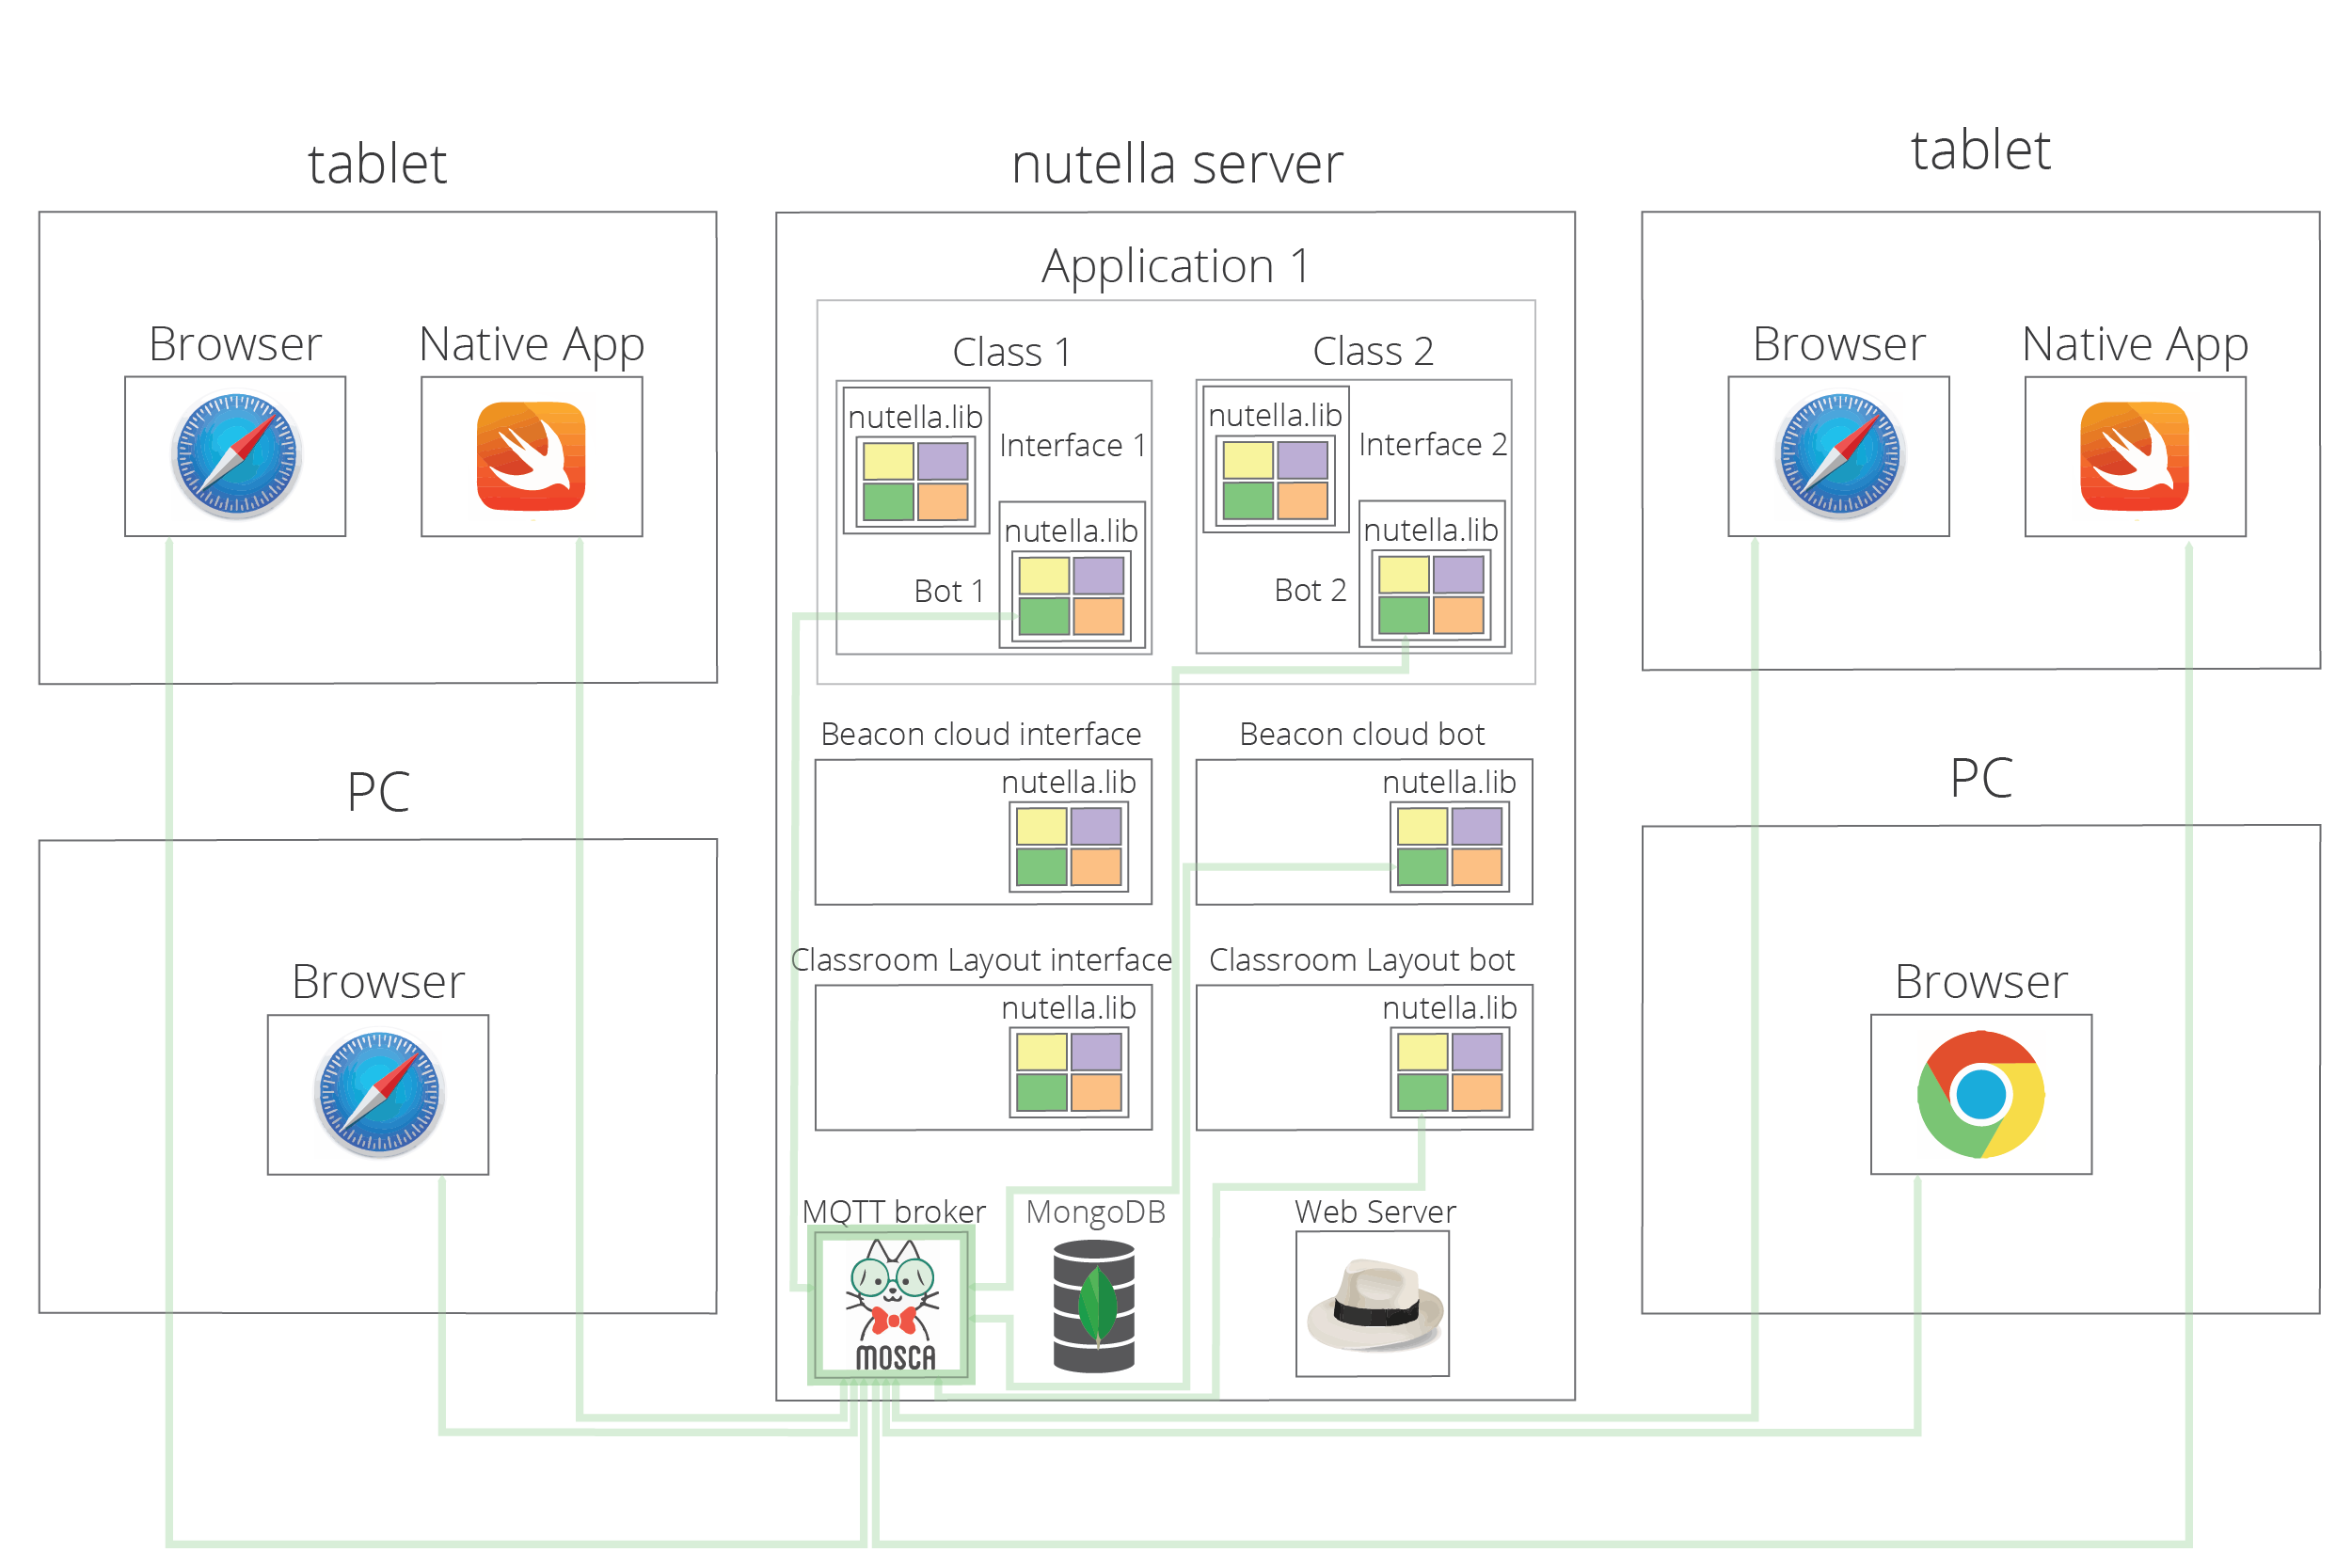
\includegraphics[width=6in]{images/nutella-client-server-broker.png}
\caption{Connections between components realized using nutella.net and internal structure of nutella server}
\label{fig:nutella_overview}
\end{figure}

\subsubsection{Nutella.persist}
This module manages automatically the data storage on the central server using different technologies. It guarantees the isolation between different instances (called \textit{nutella runs}) of the same application and it makes data persistent also when a nutella component crashes. The technologies supported are:
\begin{itemize}
\item \textit{JSON file save}: save the information on a plaintext file using the json format.
\item \textit{MongoDB}: connects to a MongoDB server instance and store data in collections.
\end{itemize}
In order to create a persisted object, the developer has only to call one of the following primitives:
\begin{itemize}
    \item \textit{Json collection store}: creates an array stored in a plaintext file.
    \item \textit{Json object store}: creates an object stored in a plaintext file.
    \item \textit{Mongo collection store}: creates an array stored in a MongoDB collection.
    \item \textit{Mongo object store}: creates an object stored in a MongoDB collection.
\end{itemize}
The name of the object is a custom string that identifies the persisted object inside the current run.

\begin{figure}
\centering
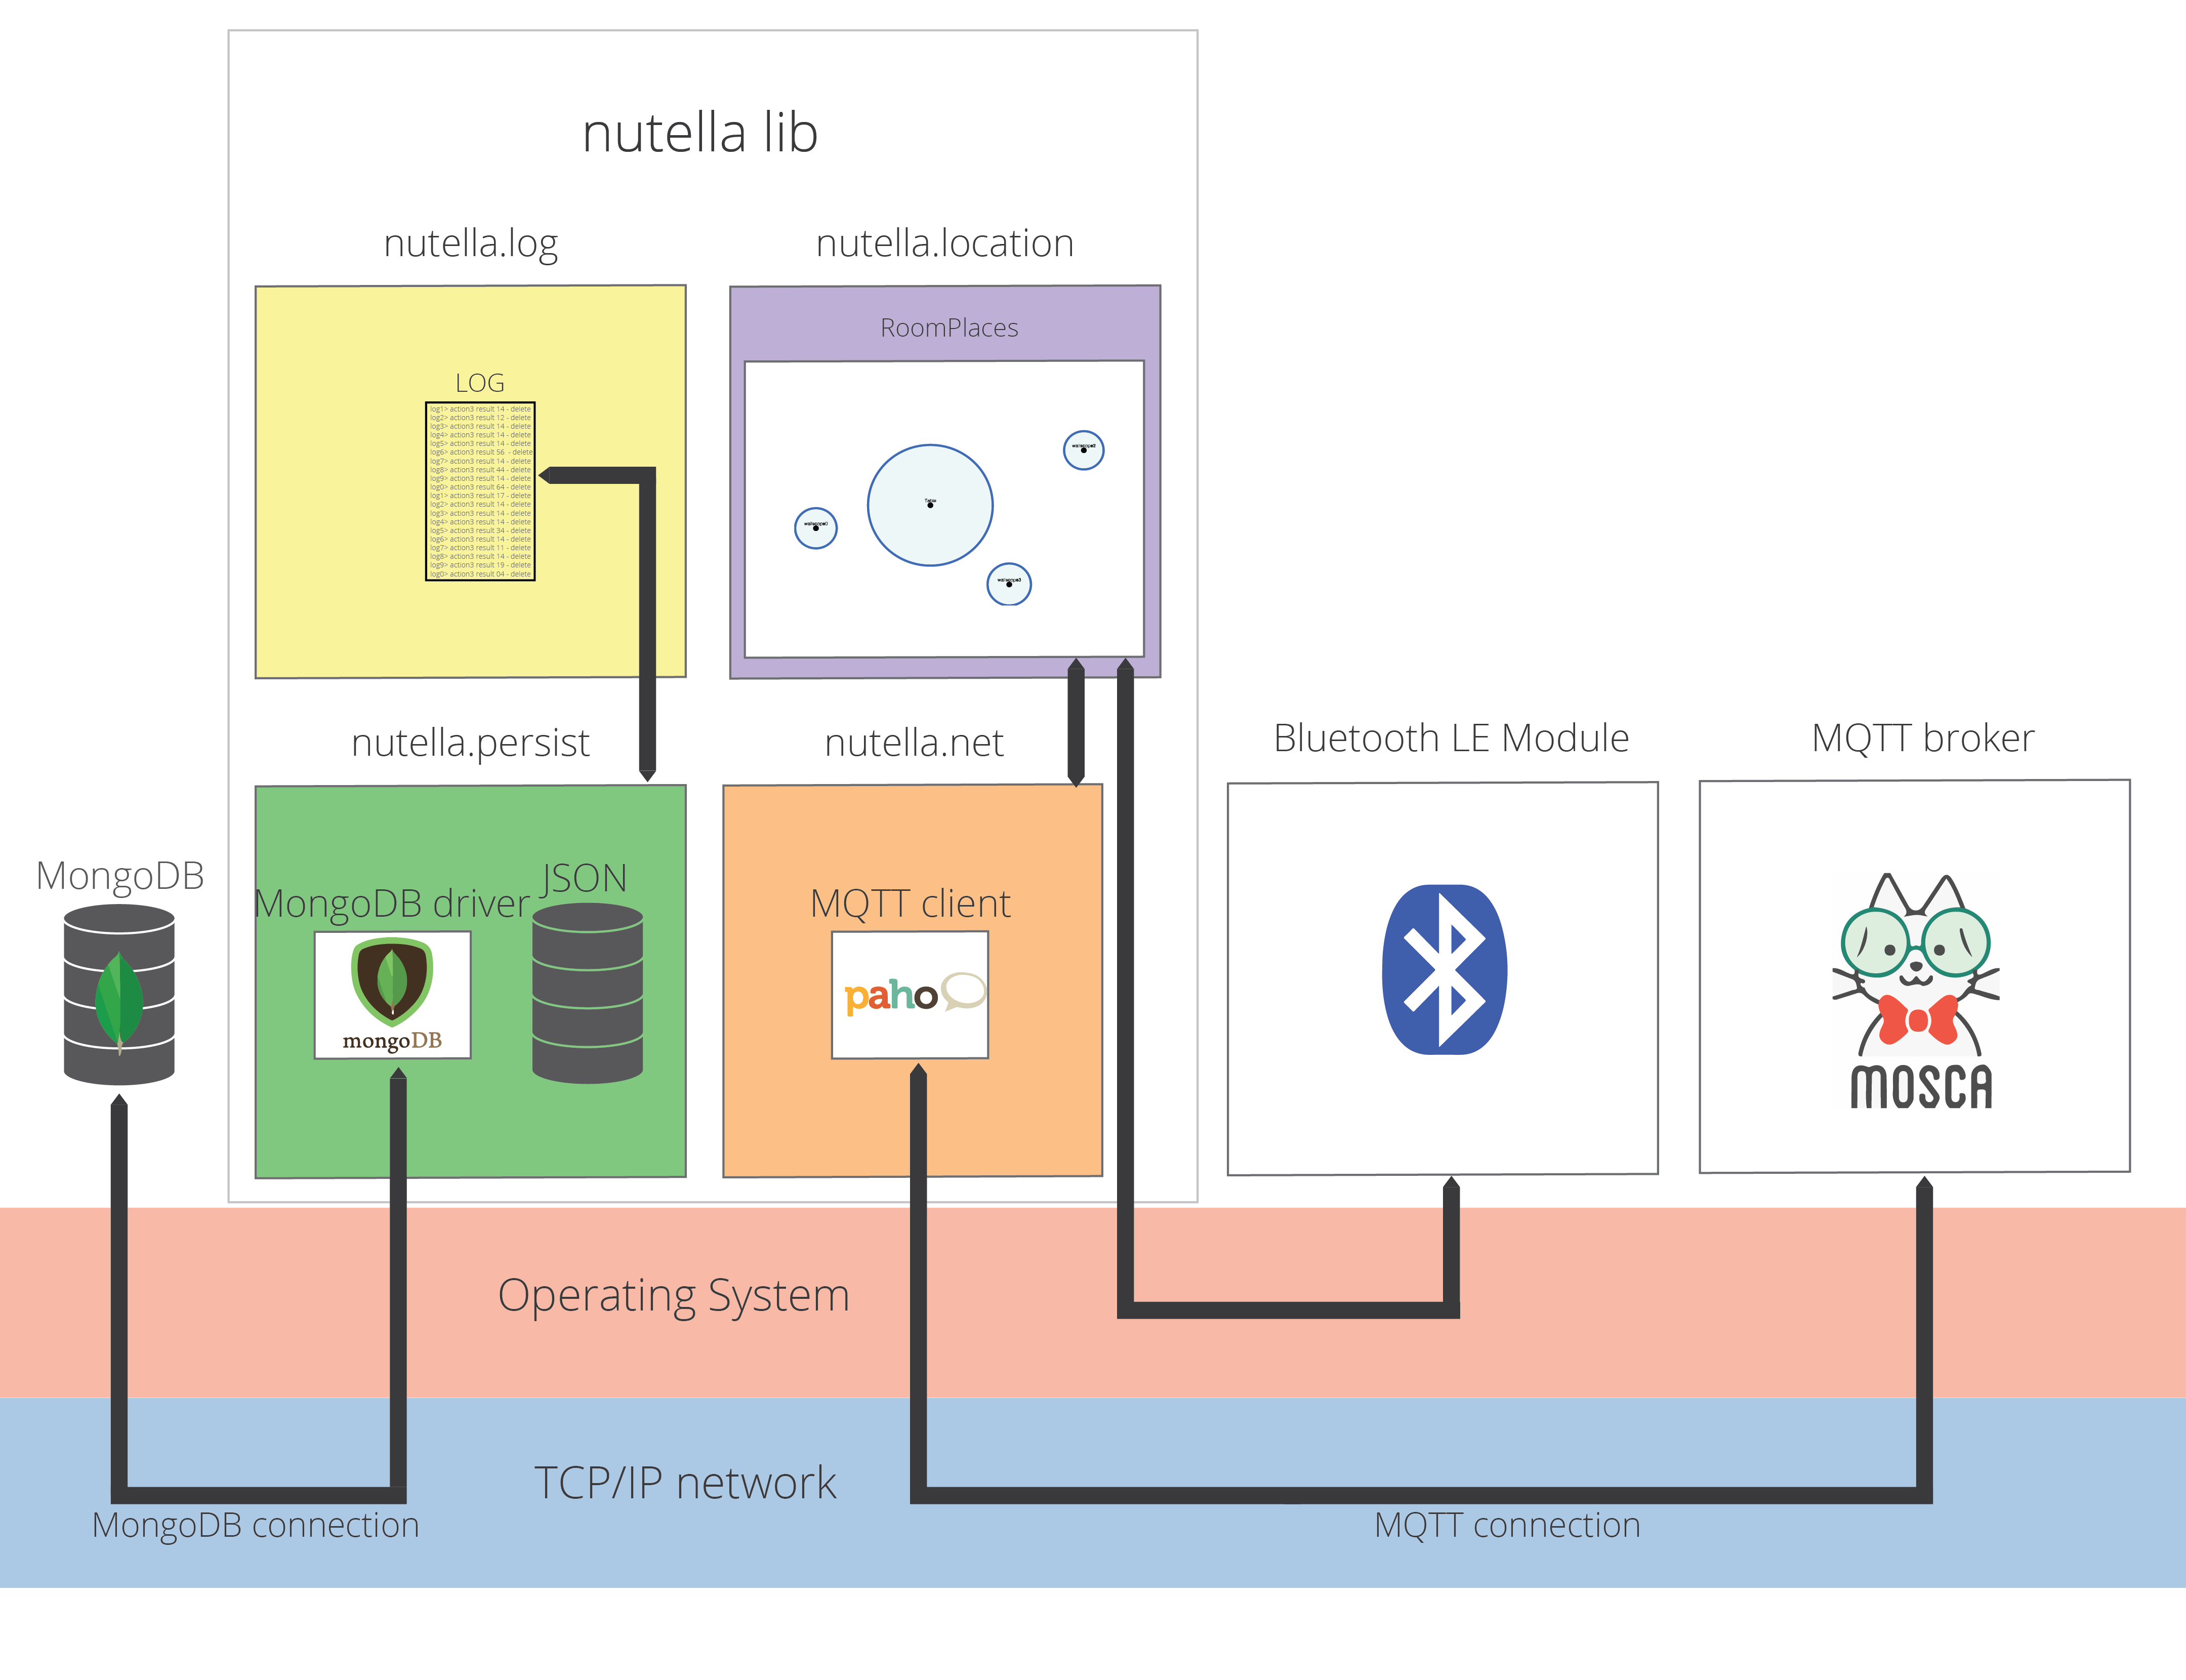
\includegraphics[width=6in]{images/nutella-overview.png}
\caption{Nutella.lib components overview}
\label{fig:nutella_overview}
\end{figure}

\subsection{Tracking system}
The tracking system is based on Bluetooth LE (Low Energy) beacon technology. I chose a specific implementation of it called Apple iBeacon because it is a mature technology compared with the others that are present on the market, it is inexpensive and guarantees the compatibility with all mobile devices that use iOS operative system and are Bluetooth LE enabled (see \ref{tab:bluetooth_le_enabled} for all the available devices). It is also easy to scale and can track a theoretical unlimited number of users, and for this reason it is suitable for many tracking applications in hospitals \cite{yang:ibeacon}, museums \cite{he:proposal}, smart buildings \cite{corna:occupancy} and lastly the \textit{Classroom of Things}.

\begin{table}
\centering
\caption{BLUETOOTH LE ENABLED iOS DEVICES}
\begin{tabular}{ | c | c | }
\hline
Device & Bluetooth LE enabled \\
\hline
\hline
iPad             & No \\
iPad 2           & No \\
iPad 3           & Yes \\
iPad Mini        & Yes \\
iPad Retina      & Yes \\
iPad Mini Retina & Yes \\
iPad Air         & Yes \\
iPad Mini 4      & Yes \\
iPad Air 2       & Yes \\
iPad Pro         & Yes \\
iPhone           & No  \\
iPhone 3G        & No  \\
iPhone 3GS       & No  \\
iPhone 4         & No  \\
iPhone 4S        & Yes \\
iPhone 5         & Yes \\
iPhone 5C        & Yes \\
iPhone 5S        & Yes \\
iPhone 6         & Yes \\
iPhone 6 Plus    & Yes \\
iPhone 6S        & Yes \\
iPhone 6S Plus   & Yes \\

\hline
\end{tabular}
\label{tab:bluetooth_le_enabled}
\end{table}

The iBeacon technology is mainly used for proximity tracking inside stores and its purpose is displaying promotions on customers’ mobile devices when the users approach a certain location in the store. 

The main hardware component of this technology is the beacon: a small device that consumes very low power and can remain active for years using a small battery. This device emits Bluetooth packets at fixed time frames, it contains an unique identifier and the calibrated RSSI (Received Signal Strength Indication) that is a parameter supplied from the constructor that allows the receiver to estimate the distance from the beacon.

Every Bluetooth Low Energy device can be a receiver component of the tracking system. The first prototype of RoomPlaces is built using iOS devices but every consideration is valid also for other mobile platforms like Android. iOS presents a native Swift API that allow RoomPlaces to query the Operative System for the nearby beacons: automatically the OS will receive all the beacon packets and will compare the calibrated RSSI field contained in the packet with the RSSI using a logarithmic model and a moving average filter for estimating the distance.

Room Places was built and tested using Estimote iBeacons \cite{estimote} with a packet emission frequency of 5Hz (one packet every 200ms) and transmission power of 4DBm, these parameters are a good trade-off between accuracy (directly proportional to the emission frequency and transmission power) and battery consumption for our application. An iBeacon configured in that way can work for six months with a single \textit{CR2477 battery} (1Ah at 3V for a total of 3Wh of energy) allowing every kind of application for one school semester.

\subsection{Integration with nutella}
RoomPlaces lives inside nutella framework, its back-end components run on the server as nutella bots and its interfaces are accessible using a browser through a web server called Sinatra (that is part of nutella framework and is illustrated in \ref{fig:nutella_web_server}). This is an high level description of how the framework works. When the developer creates a new application nutella will generate empty bots and interfaces directories. Bots are back-end programs that run on the central server and interfaces are web pages that are transmitted to the client and run inside the client browser. The development  process of an application consists is inserting code inside bots and interfaces in order to generate the desired behavior of the application. For lunching multiple instances of the created application is necessary to use the command \textit{nutella start run\_id}, where the run\_id is the name of the new instance of the application (for example the name of the class in which the application will run). Every instance of bot can be used in only one class, there's not theoretical limit on the number of instances that can be created. The framework will ensure the isolation between classes and guarantees that every change on the state of one class will not be reflected in the other classes. It is important to highlight that in nutella architecture the code is shared between all the instances, but the state is saved on plaintext files or inside a MongoDB collection in a separated directory and for this reason it is possible to update the code and modifying the data independently. It is also possible to update the code and replace run-time some bot instance without suspending the exectution of the others.

\begin{figure}
\centering
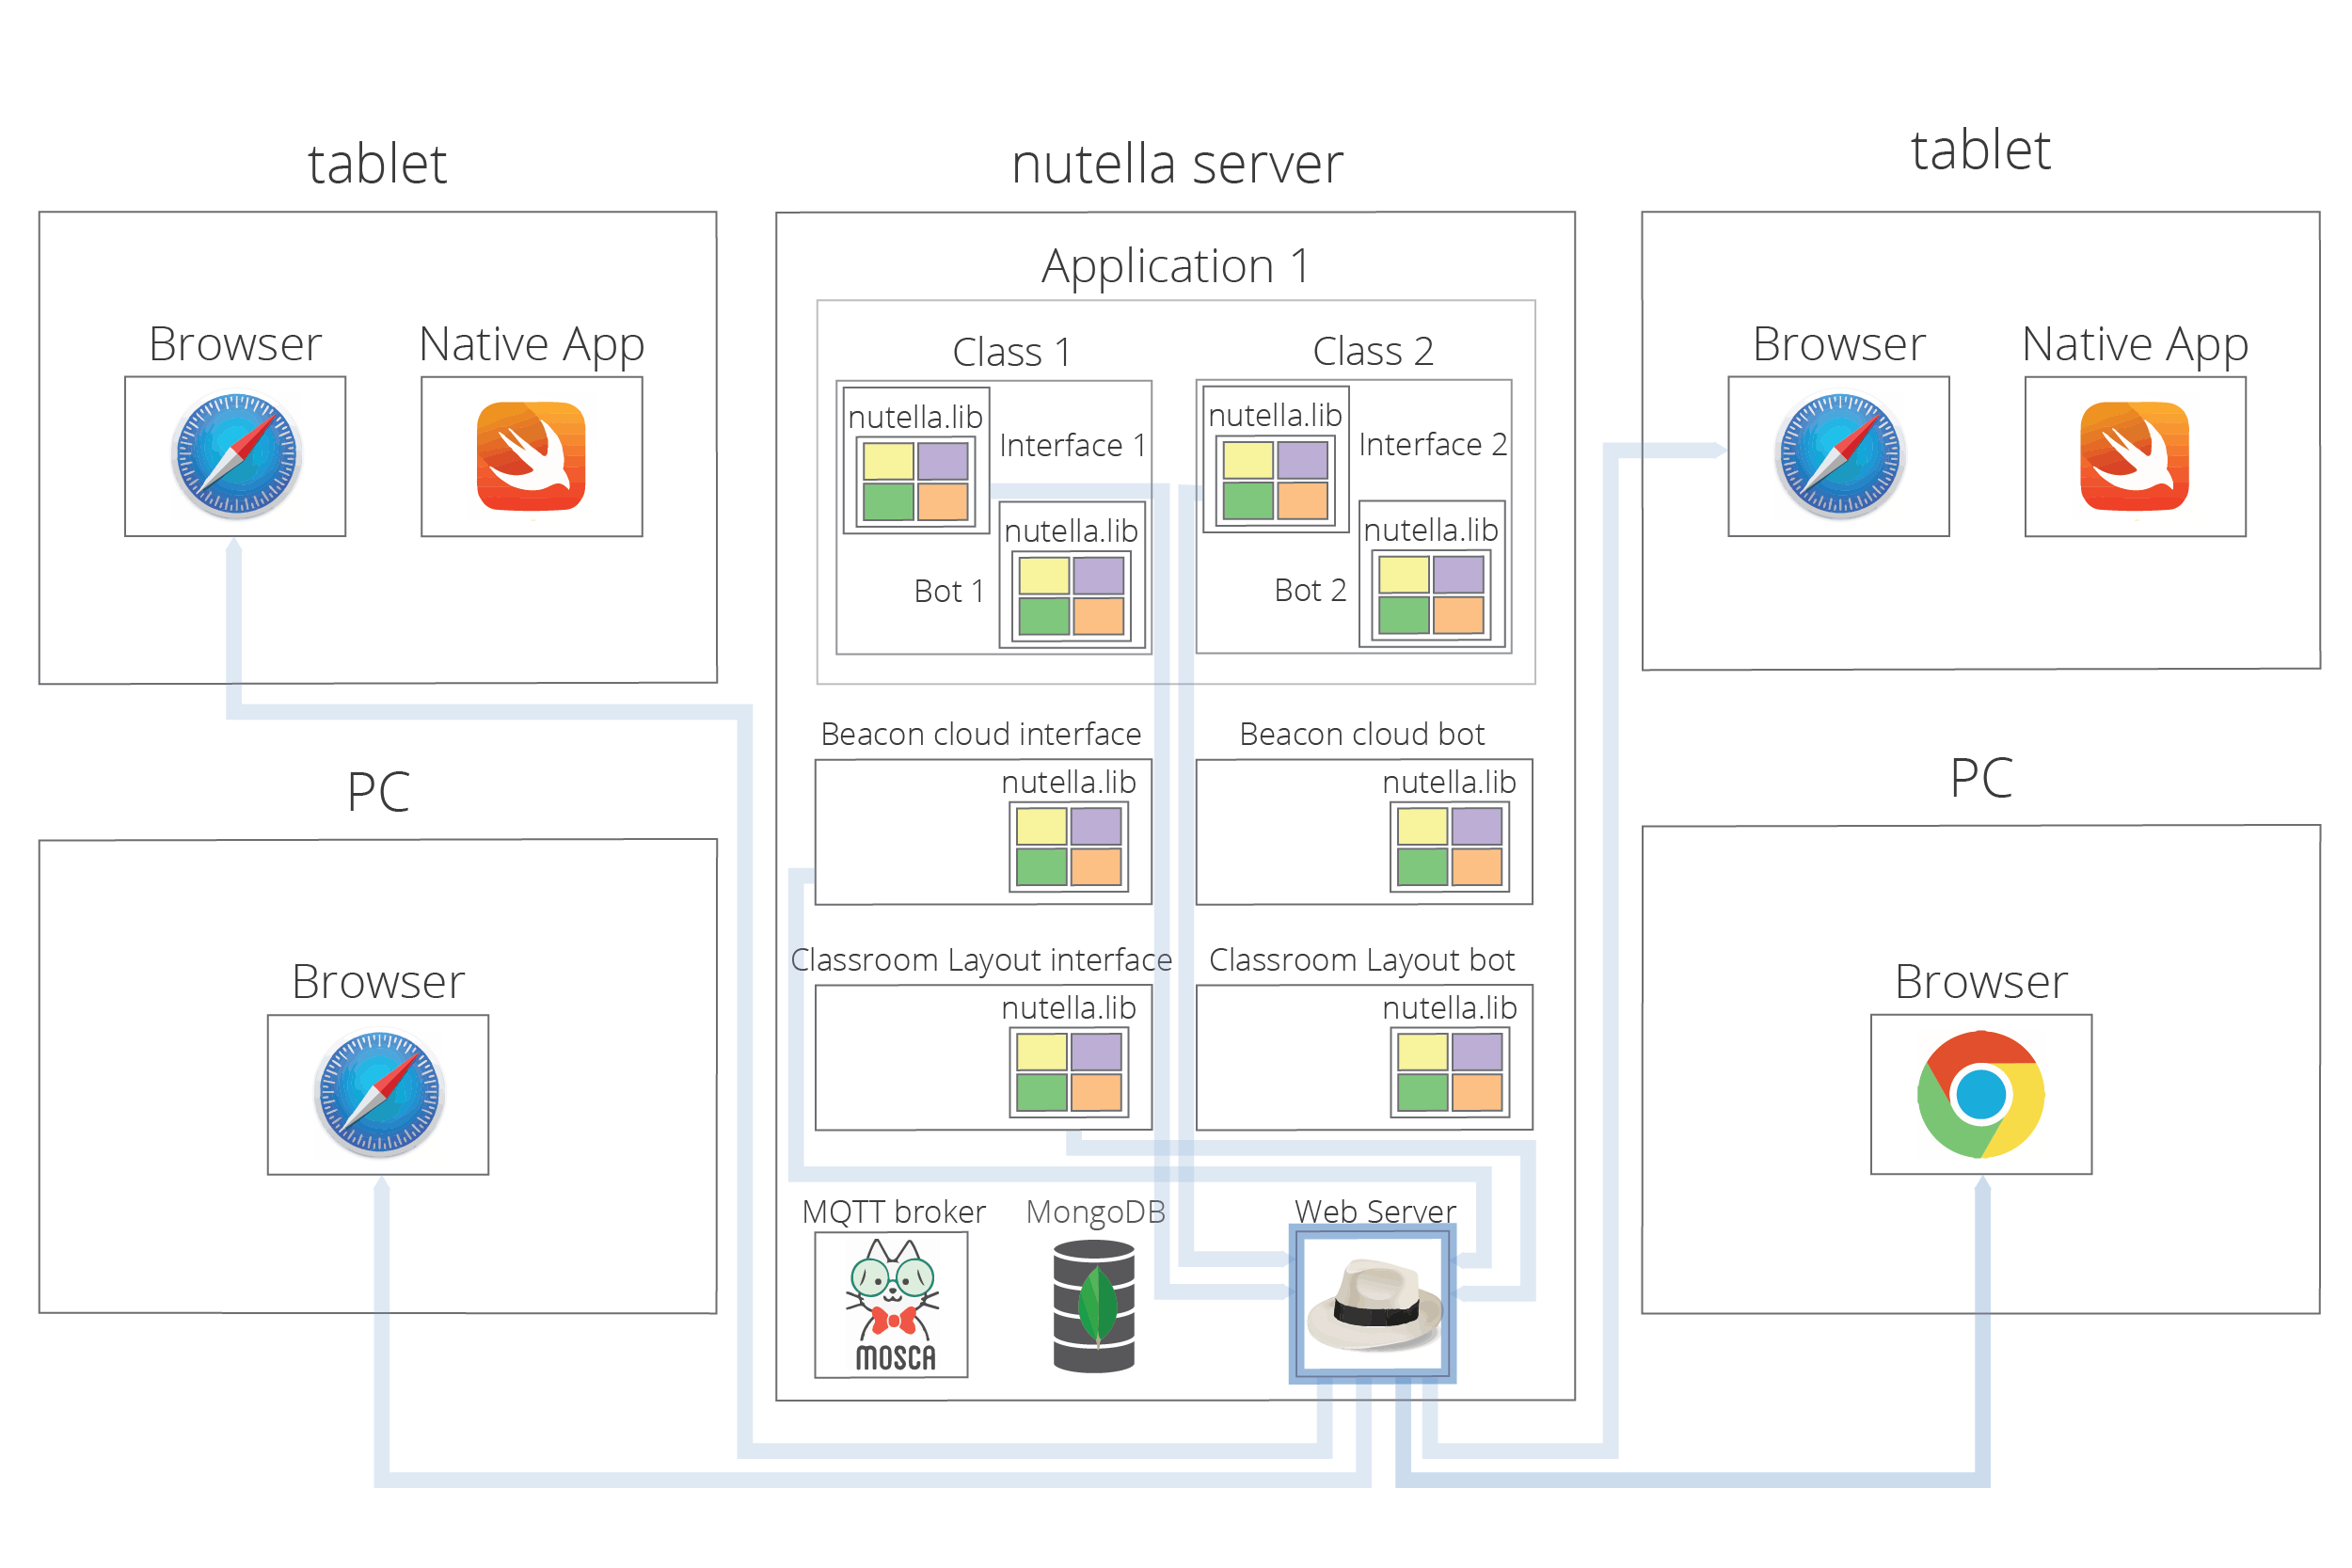
\includegraphics[width=6in]{images/nutella-client-server-webserver.png}
\caption{Nutella interfaces distributed though Sinatra web server integrated in \textit{nutella framework}}
\label{fig:nutella_web_server}
\end{figure}

\subsection{RoomPlaces definitions}

RoomPlaces main purpose is tracking \textit{resources}. A \textit{resource} is an entity in the 2D classroom space, it can be a \textit{beacon} or a \textit{mobile device} (tablet or phone) and it is identified by an unique \textit{RID} (Resource Identifier, an alphanumeric string) assigned by the developer. There are two types of resource: \textit{static resource} has a fixed position and it is used as a reference point for tracking other resources, \textit{dynamic resource} can move: its movement can be manipulated using the APIs (contained in nutella.location) or automatically tracked. Static resources have a proximity radius that is the maximum distance in which they can sense other objects, everything farther than that is ignored.

There are two types of coordinate systems supported by Room Places: continuous and discrete. They can coexist in the same room and every static resource belongs to one of them. The axis on the discrete coordinate system can be both configured for expressing the coordinates with integer numbers or letters.

Dynamic resources can be manually positioned using one of the two coordinates systems (through RoomPlaces APIs) or can be automatically tracked using the proximity tracking system. In the latter case the position is automatically assigned if the resource is close enough to a static resource. For determining the proximity, the estimated distance between the dynamic and the static resource is compared with the static resource radius.

\subsection{Core components}
The most important component of Room Places is called \textit{RoomPlaces Bot} and at every time there's one instance running that serves multiple classes at the same time. Nutella framework bots are special back-end components that are instantiated only once during the nutella startup procedure and are always running in background. This component translates a stream containing distances between static and dynamic resources (generated by mobile devices) into an high level representation of the classroom resources. There are two functionalities provided to other components: a query system and a push notification service. The first one allows a component to request the position of a resource at any time (pull functionality) and the second allows a component to subscribe to a specific event (related to the proximity of resources) and be notified every time that the event occurs (push functionality). All the components are illustrated in \ref{fig:nutella_web_server}.

\subsubsection{Classroom Layout}
\textit{Classroom Layout} is a nutella interface used in order to configure RoomPlaces Bot. It is a static web page that communicates with the Bot and it allows the user to create resources, configure the role (static or dynamic) and the coordinate system that is desired (continuous, discrete or automatic proximity tracking). This interface is designed for being used by developers but also in the future by teachers that will include the tangibles that are present in their classroom.

\subsubsection{Beacon Cloud}
\textit{Beacon Cloud} is a nutella interface used for adding beacons to the set available in Classroom Layout. This interface (shown in \ref{fig:wallcology_beacon_cloud}) associates three numbers that are needed for identifying an iBeacon (UUID, major, minor) with the RID that is assigned to it. The numbers are inserted only once when the beacons are purchased. The beacon information is stored into a component called \textit{Beacon Cloud Bot} that has the capability to be queried for the list of all beacons present in the system (needed by the iPads that need to identify if nearby beacons belongs to the system or not).

\subsubsection{RoomPlaces Location Tracking}
\textit{RoomPlaces Location Tracking} is part of the standard nutella library (module \textit{nutella.location}) and is available on mobile platforms. It is implemented in Swift for running on iOS operative system is packaged as an iOS framework that can be easily included in any application. An instance of it runs on every iPads and iPhones. It contains the routines that query the operative system for the beacons physically around the device and compare the beacon identifiers (UUID, major and minor) with the values contained in Beacon Cloud Bot list in order to understand if a relevant beacon is found. The output of this component is a list of beacons with the relative distance from the device where the software is running. It communicates this list to Room Places Bot every second: iOS APIs update the list with 1Hz frequency and for this reason the delay of the tracking system cannot be lower than 500ms in average, 1000ms in the worst case. When the device is configured as a dynamic resource (the software must query Room Places bot for discovering this information), Room Places Location, will request Beacon Cloud for obtaining a virtual beacon identity and will start broadcasting beacon packets. Every time that Beacon Cloud creates a virtual beacon it informs all the components that a new beacon is present in the system and from that moment on they can start tracking it. This process is completely transparent to the developer.

\subsection{RoomPlaces communication protocol}
For allowing RoomPlaces components to communicate it is necessary the sets of rules described in the the open-source RoomPlaces protocol. It is a message oriented protocol based on nutella protocol: every message is encapsulated inside a nutella message and sent over the network taking advantage of the nutella connection (it uses MQTT protocol and eventually websockets when running inside browsers). This choice enables to use the set of network abstractions provided by nutella: the \textit{push/pull} communication methods over channels, the isolation between different instances of the same application (running in different classrooms), the automatic server address discovery and connection management (for automatic reconnection). The protocol is described in details in \autoref{apdx:roomplaces_protocol}.

\subsection{Application Programming Interfaces}
On top of this existing layer of technology sits an abstraction layer provided by RoomPlaces, what I call the APIs layer \cite{nutella_location}. Its goal is providing an easy access to RoomPlaces functionalities, enabling the developer to interact with all its components without knowing RoomPlaces protocol. The APIs are consistent over all the platforms and implemented inside \textit{nutella.location} module.

There are two main functions inside the APIs: the first is retrieving resource objects and read/write configuration parameters on them as they were local objects, this is a \textit{pull} functionality because it allows the developer to know the state of one resource at any time. The synchronization mechanism (with the other RoomPlaces components) is voluntarily hidden, there's no need to explicitly tell when to send or load data on the server. The second functionality is subscribing to specific events; this is a \textit{push} capability because it notifies the application when the event occurs without the need to constantly query the server looking for changes. The supported events are generated by dynamic resources that enter or exit the range of a static resource. This is the effective mechanism that implements the \textit{event stream} and allows a lightweight interaction with tangibles when the goal is sensing the proximity between objects.

In order to implement the \textit{tangible containers} (storing information inside physical objects) every resource object retrievable using the API has a set of key value pair. Adding or modifying a key value pair will automatically insert the data inside the object and propagate the modifications to the whole system (saving the permanently the data on the server).

This set of APIs is designed keeping in mind the iterative nature of the macroworld development process: there's a feature that I call \textit{continuous resource update} that allow the resource object list present in the API to continuously listen for resource updates. The consequence of this feature is the possibility of adding, removing and modifying resources without the need of restarting all the other components and request updates to the server at fixed time interval. Another effect is that every resource object inside the list is constantly up to date (when position or other parameters change) reducing the query delay (compared with the standard client-server implementations where a remote component must be called every time a get request is executed). The \textit{continuous resource update} is implemented with a push mechanism: every client is waiting for updates subscribing to a nutella channel (using the \textit{subscribe} primitive provided by \textit{nutella.net}), when an object is modified an alteration message is sent and is instantly propagated through the network. In order to increase reliability all the alteration messages are checked by \textit{RoomPlaces Classroom Layout} component and not propagated to other components in case they contain errors. A detailed explanation of the RoomPlaces APIs can be found in \autoref{apdx:roomplaces_api}.

\subsection{RoomMonitor}
It is another part of nutella framework and it is developed in order to enable the developer to inspect components of the system, discover problems and send alert messages in case of crashes. The first goal is achieved using the interface visible in \ref{fig:nutella_monitor} that displays the components in a circle where arcs represent component and are proportional to the number of channels that are used by that component. Connections between components are visualized with white lines. It is also possible to show all the messages sent on every connection clicking on the links. The second function of this component is: enable the system administrator to insert an e-mail to be notified every time a system component crashes. This function is useful while the system is running inside classrooms because it provides instant feedback when something goes wrong. The application instances that run into classes can be inspected singularly using the selection menu on the left of the interface. The number of problems are also reported (in the orange circle) in order to quickly see the state of every classroom instance.

\begin{figure}
\centering
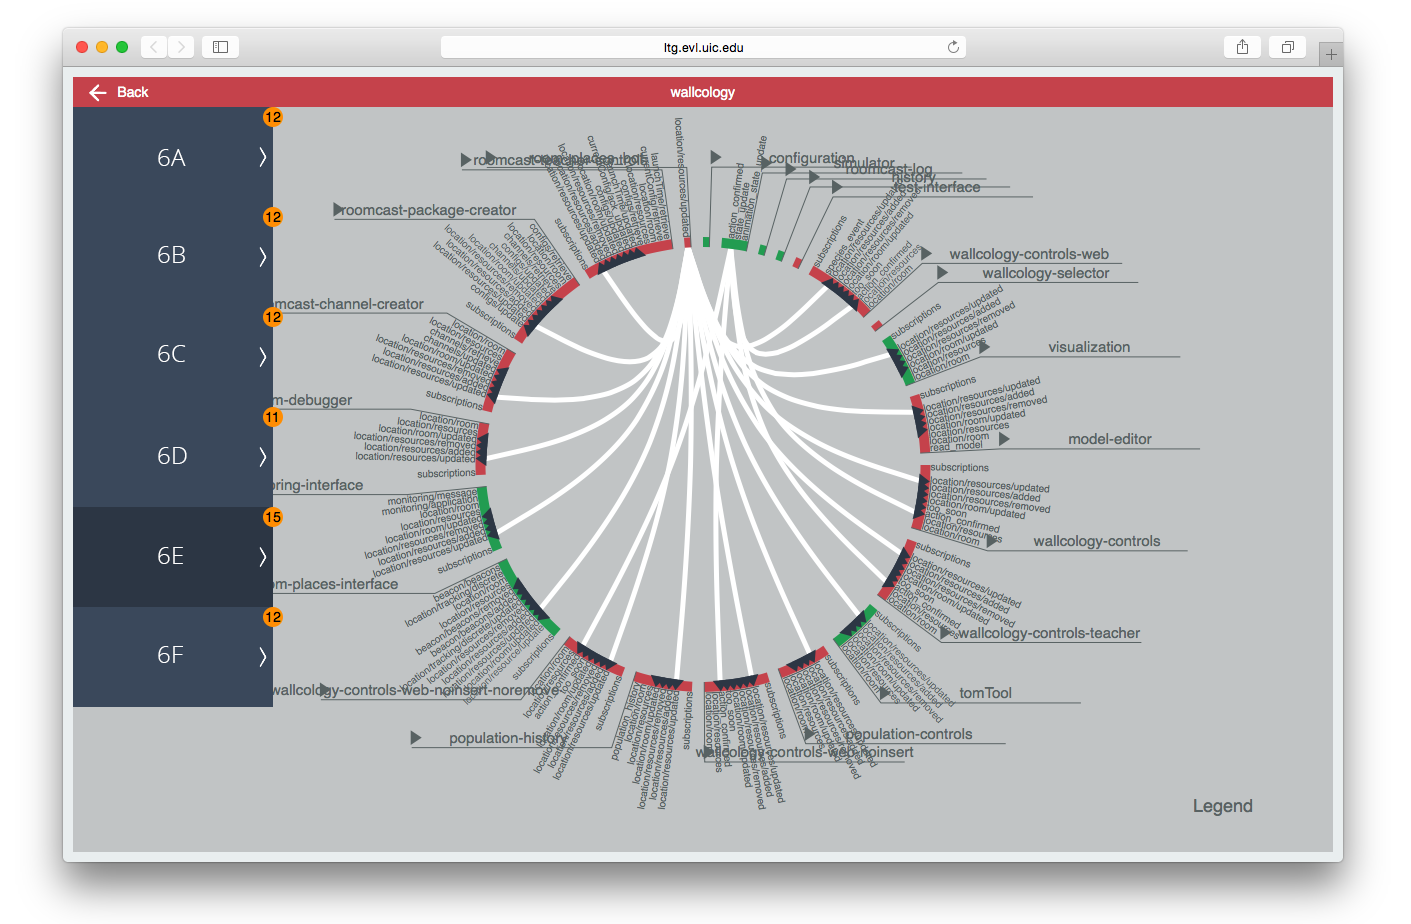
\includegraphics[width=6in]{images/nutella-monitor.png}
\caption{Nutella RoomMonitor interface. On the left there's the menu for selecting the classroom instance, on the right the components disposed in circle and wired using nutella channels represented with white lines.}
\label{fig:nutella_monitor}
\end{figure}

\section{Configuration environments}
Inside RoomPlaces there are two configuration environments that allow the software developer to describe the physical room and assign name and roles to objects. Every configuration environment is composed by one interface and one bot already explained in the previous section. In this section I describe how bot and interface work together during the configuration of the system. The first environment is Beacon Cloud, it is a list of beacons that will be used inside classrooms, the interface is unique for all the classrooms since the technical characteristics of the beacons remain the same (UUID, Major, Minor). The second interface is called Classroom Layout and is different for every class. It shows the objects that are tracked inside the classrooms and allow to chose name and roles. Both of them are accessible on the nutella landing page (that is personalized based on the class).

\subsection{Beacon Cloud}
It is a web interface (\ref{fig:wallcology_beacon_cloud}) created with the purpose of being the only point in the system that deals with the technical details of beacons. It has a table that contains all the physical beacons that are used in classrooms and for every one of them the RID and three numbers that uniquely identify it: UUID (Universally Unique Identifier), Major and Minor. For inserting a new beacon there's an empty line at the bottom, basic integrity checks are executed in order to ensure that the input is valid. There's also the possibility of changing parameters for a beacon already present in the list. All the changes are propagated real-time to all the other components of the system: this feature allows the developer to continuously add, remove and modify beacons during the development phase.

\subsection{Classroom Layout}
It is the main configuration interface for RoomPlaces. The purpose of it is allowing the user to insert all the physical resources that must be tracked inside the virtual space. It is composed by two graphical components: on the left there's a map of the classroom that shows the resources already present with their names. It is also possible to change the room dimensions modifying the quotations.

\begin{figure}
\centering
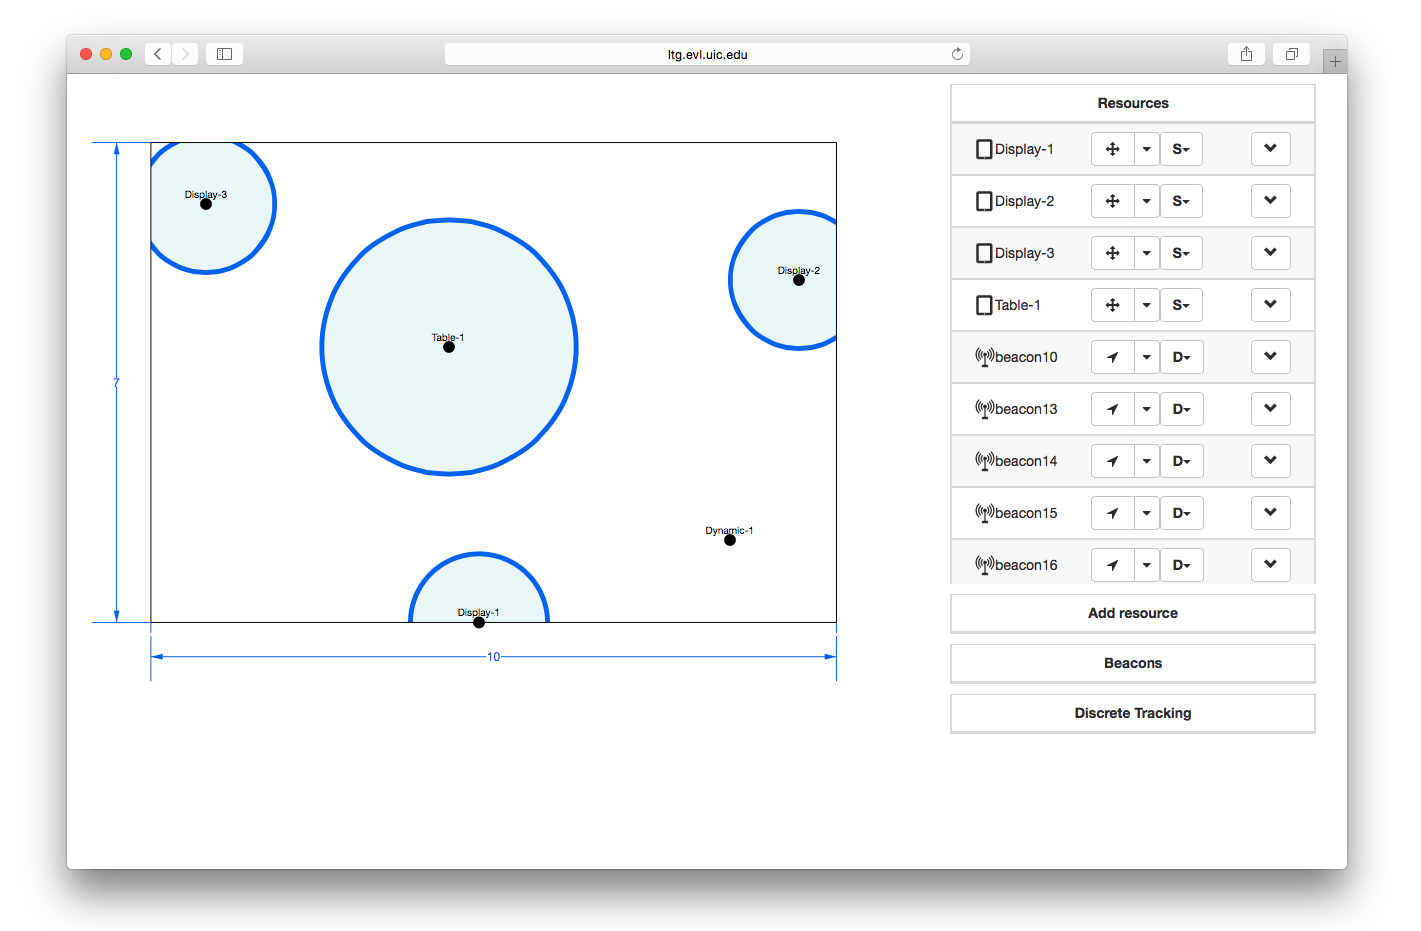
\includegraphics[width=6in]{images/classroom-layout-map.png}
\caption{Classroom Layout interface with the typical scenario configuration}
\label{fig:classroom_layout_map}
\end{figure}

On the right side there's a menu with add, remove and edit functions. It is divided in four sections as shown in \ref{fig:classroom_layout_map}. The first section list all the resources that are already tracked in the class, for every resource is possible to configure the coordinate system (continuous or discrete) and the role of the resource (static or dynamic). Expanding the menu contained in every resource, a number of additional parameters appear: position in the 2D space according to the chosen coordinate system, proximity radius for static resources and a set of key-value pairs that allows to insert information associated with that resource.

\begin{figure}
\centering
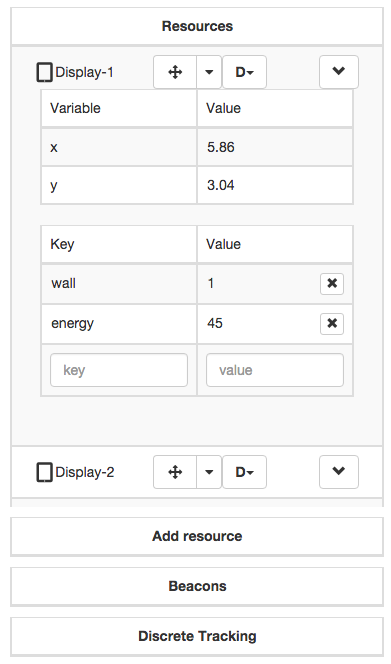
\includegraphics[width=1.9in]{images/classroom-layout-resources.png}
\caption{Resources menu that allows to modify the parameters of resources in the system}
\label{fig:classroom_layout_resources}
\end{figure}

The second (\ref{fig:classroom_layout_add}) section is used for adding a new resource: it allows to chose the type of device, the coordinate system used and the role. 

\begin{figure}
\centering
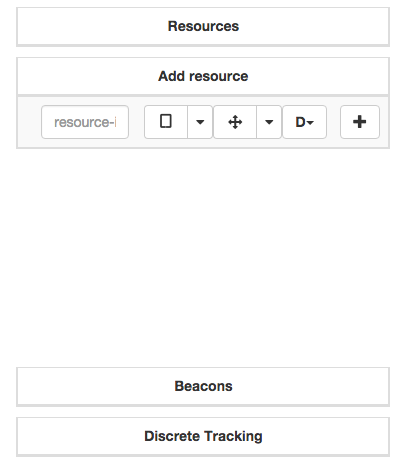
\includegraphics[width=1.9in]{images/classroom-layout-add-resource.png}
\caption{Add resource menu that allow to insert new resources to the system}
\label{fig:classroom_layout_add}
\end{figure}

The third (\ref{fig:classroom_layout_beacons}) allows to pick a beacon from the list provided by Beacon Cloud, clicking on the add button the beacon will automatically be configured as dynamic resource automatically tracked in continuous coordinate system.

\begin{figure}
\centering
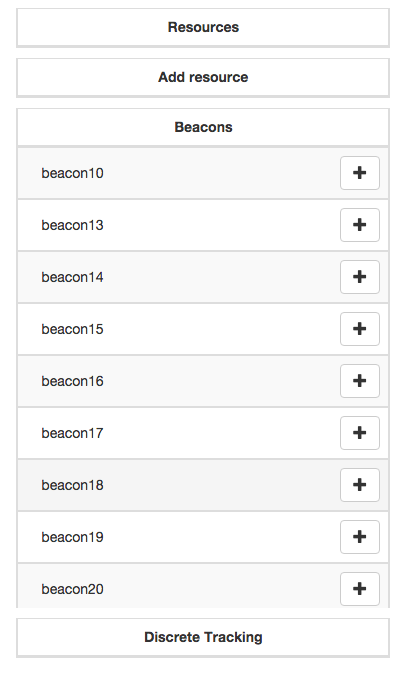
\includegraphics[width=1.9in]{images/classroom-layout-beacons.png}
\caption{Beacons menu that allows to insert beacons resources that are already in Beacon Cloud list}
\label{fig:classroom_layout_beacons}
\end{figure}

The last section in the menu (\ref{fig:classroom_layout_discrete}) is dedicated to the configuration of the discrete tracking system. Since this system coexists in the same room at the same time with the continuous one, it is possible to map one over the other. The user can control every aspect of this mapping, inserting continuous coordinates and dimensions of the discrete tracking system external rectangle and the number of cells. The other configuration parameter is the possibility of expressing discrete coordinates with letters or numbers, this possibility is introduced in order to minimize the possible errors when the users have to auto report their location.

\begin{figure}
\centering
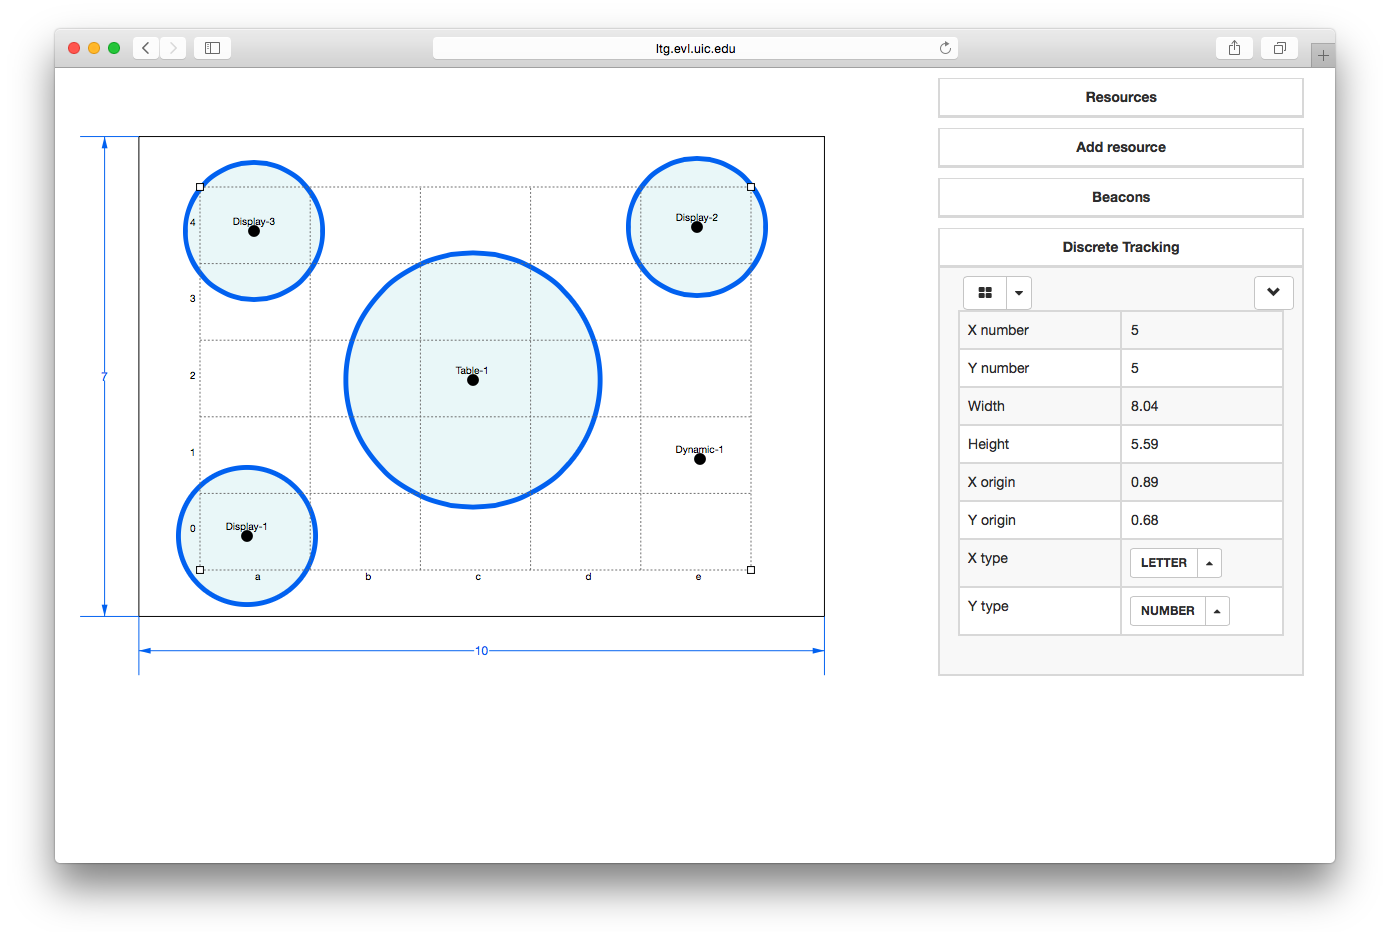
\includegraphics[width=4.5in]{images/classroom-layout-discrete.png}
\caption{Discrete coordinate system represented on the map. When the coordinate system is modified also the resources that use it are moved accordingly on the map.}
\label{fig:classroom_layout_discrete}
\end{figure}

The map always displays in real time the state of the classroom. It is possible to drag and drop all the static resources for changing position. Every one of them has a proximity radius represented with a blue circle. All the dynamic resources with distance lower than the radius are considered in proximity of it. Dragging the radius on the map will modify that parameter according to the graphical representation. On the map in \ref{fig:classroom_layout_discrete} is also displayed the discrete coordinate system and the resources that use it, on the edges there are signifiers (little squares) that can be moved for modifying the shape of the external rectangle. The map is useful also for debugging purposes: every time a dynamic resource is considered in proximity of a static resource it is displayed using a circle with a radius equal to the estimated distance. 

\section{Tangible interface development with Room Places}
The framework components described above, together with nutella framework, were designed for supporting the entire development process of new applications (macroworlds) that take advantage of tangible interfaces for interacting with the simulation. I will go through every phase of the design and I show how the different parts of RoomPlaces support the developer in those phases. In the next chapter, I will go into more detail and provide specific examples of how RoomPlaces addresses the challenges described in \autoref{chap:lit_rev}.

\begin{figure}
\centering
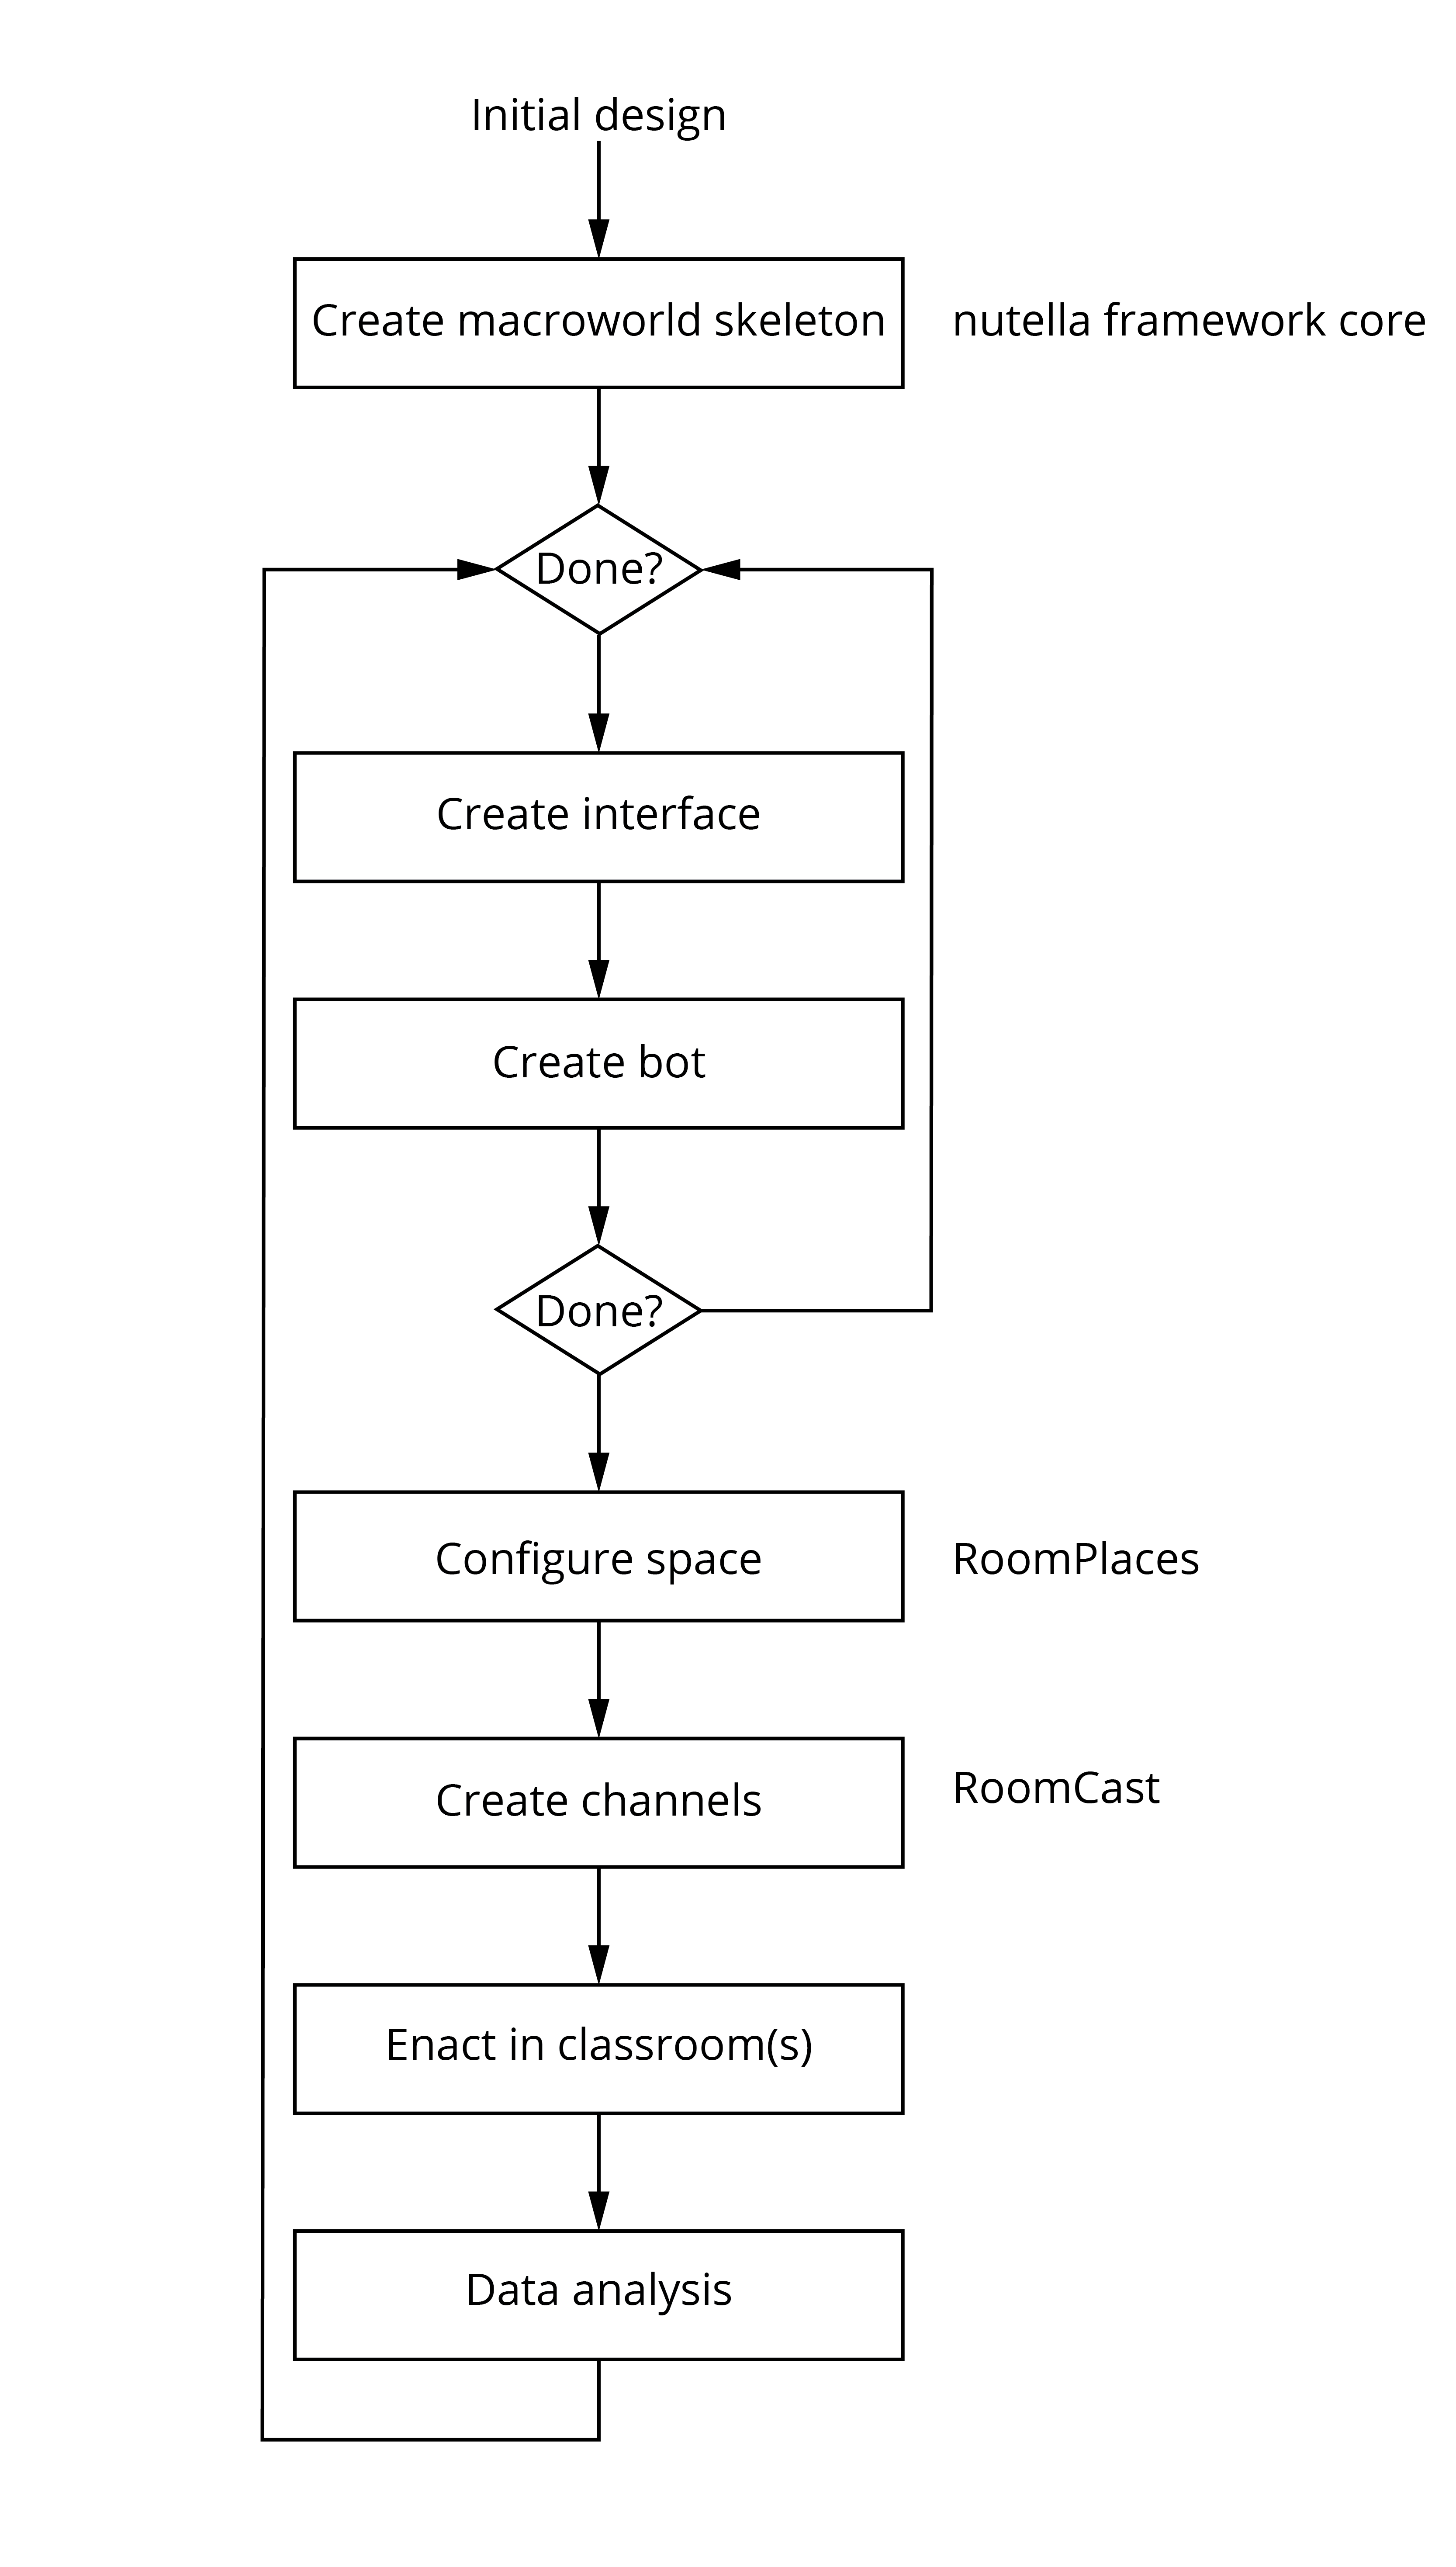
\includegraphics[width=3in]{images/nutella_workflow.png}
\caption{Macroworld design and implementation general workflow with nutella and RoomPlaces}
\label{fig:nutella_workflow}
\end{figure}

\subsection{Initial design and beacon purchasing}
The first step in designing a macroworld application is to decide what to build. It is important to point out that the design and development processes are tightly coupled and highly iterative. RoomPlaces \textit{continuous resource update} capability was designed for supporting this process allowing the developer to start and stop components as well as adding, removing and modifying resources without worrying about the synchronization with the server (that is totally transparent when using the APIs).

RoomPlaces is one of the components needed to design a macroworld, for this reason it is useful to contextualize it inside the nutella application design. In the \ref{fig:nutella_workflow} there's an overview of the entire development process using nutella. It is useful to observe the \textit{space configuration} step that involves RoomPlaces is repeated many times until the desired result is obtained and the application meets all the goals of the developer, for this reason several iterations must be supported and no hypothesis can be done on the order of the actions that must be executed on the configuration interfaces.

After the initial design is known, the designer must decide what are the interactions that can be supported with a tangible interface. No assumptions were made in RoomPlaces on the number of resources and the dimension of the tracked space, the limit is the creativity of the macroworld designer. After the initial tangible interaction has been designed it is necessary to build or buy beacons. The beacons can be shared among classrooms, minimizing the number of beacons that are needed. The suggestion in this phase is to always buy more beacons than needed, this is for replacing beacons that are broken during the application execution. This replacement is supported by RoomPlaces and can be done on the fly, thanks to \textit{continuous resource update}, without restarting any component.

\subsection{Environment configuration process}
When the beacons specifications (the three numbers that identify every one of them) are known it is necessary to insert them in \textit{RoomPlaces} using the \textit{Beacon Cloud} interface. All beacons are inserted in this cloud regardless their constructor and from this point on they will be referenced using the name inserted in \textit{Beacon Cloud}. From this interface is possible to add or remove beacons in successive iterations.

For configuring what objects have to be tracked there is the \textit{Classroom Layout} interface that allows the developer to insert beacons from a list (the \textit{Beacon Cloud} list). From this interface is also possible to insert resources with an arbitrary name into the room and assign a position to them. It is also useful for debugging: every time that a dynamic resource is detected it is automatically displayed on the map. This feature allows the developer to start testing the configuration before writing the first line of code. It is also useful during the development phase of every cycle because it is possible to see arrival and departure events without the need of writing an external logger for them. As the previous interface also Classroom Layout will remain available all the time during the development. Those modifications can be done on the fly (without requiring a restart) for supporting incremental application development of more components of the system.

\subsection{Code development process}
This is the process that takes the specifications and translate them into components of the macroworld. Every programming language is supported in this phase because all the protocols used are open-source, although the nutella library is already provided in JavaScript, Ruby and Swift languages because past experiences in macroworld development suggested them as most popular languages.

There are two methods for interact with RoomPlaces: using the APIs provided in nutella library and make requests and subscriptions directly to \textit{RoomPlaces} bot using \textit{nutella.net} or directly an MQTT client library. The fist is simpler and requires the programmer to call only functions already implemented taking advantage of the layer of abstraction that APIs provide. The latter is useful in the scenarios where a component has to be implemented in a language in which nutella library is not provided. If the developer choose this option it is necessary to understand  RoomPlaces protocol and how the components are wired together using nutella network library (\textit{nutella.net}).

If the developer decide to use the APIs, all the needed tools are provided inside functions and data structures of \textit{nutella.location}. The most important data structure for bootstrap the components is \textit{nutella.location.resources}: it is an array of resources that can be used in every moment for accessing object properties in the room like tracked location and stored parameters. It is also possible listen to arrival and departure events. For all the technical details see \autoref{apdx:roomplaces_api}.

After some iteration, when the code is developed and tested, is time to deploy the application inside the classrooms. For doing it is necessary to use the command "\textit{nutella start runid}" on the server that creates a new instance of the application. When a new application instance is created, every bot is instantiated and wired with the other components. During the time in which the application is running, RoomPlaces \textit{Classroom Layout} interface can be used for looking how resources are moving in the class and for detecting eventual anomalies. In order to monitor the general behavior of the application, how components are wired together and if some component crashed, it is possible to use \textit{RoomMonitor} interface that entirely developed for this purpose and shown in \ref{fig:nutella_monitor}.
